%\begin{tikzpicture}
%
%\draw[->] (-2,0) -- (3,0);
%\draw[->] (0,-1) -- (0,3);
%
%\draw[->,line width=0.5mm] (0,0) -- (-1,2);
%\draw[->,line width=0.5mm] (0,0) -- (2.24,0);
%
%\draw[dashed] (-0.44,-0.9) -- (1.34,2.68);
%%\draw[->,line width=0.5mm] (0,0) -- (-0.9, 0.44);
%%\draw[->,line width=0.5mm] (0,0) -- (-1,0.61);
%\draw[->,line width=0.5mm] (0,0) -- (1,-0.61);
%
%
%
%
%
%\filldraw[red, opacity=0.5] (0,0)--(-0.1467,-0.3000) arc (240:330:.3339) -- (0,0) ;
%\draw[black, opacity=1] (0,0)--(-0.1467,-0.3000) arc (240:330:.3339) -- (0,0) ;
%\filldraw(0.04,-0.2) circle (.02cm) ;
%
%%Beschriftung
%\draw (3.4,-0.1) node {$x_1$};
%\draw (-0.1,3.3) node {$x_2$};
%
%\draw (.45, -.6) node {$v$};
%\draw (-.25, 1) node {$x$};
%\draw (1,0.3) node {$Hx$};
%
%
%\end{tikzpicture}

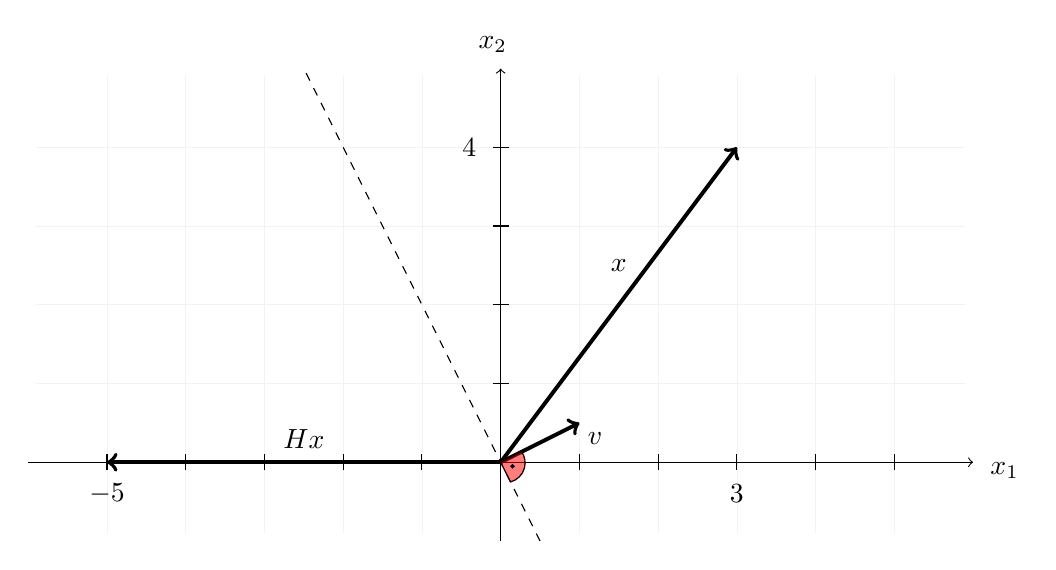
\begin{tikzpicture}
\draw[step=1,gray,very thin, opacity=0.1] (-5.9,-0.9) grid (5.9,4.9);

\draw[->] (-6, 0) -- (6,0);
\draw[->] ( 0,-1) -- (0,5);
\draw (1,-.1) -- (1,.1);
\draw (2,-.1) -- (2,.1);
\draw (3,-.1) -- (3,.1);
\draw (4,-.1) -- (4,.1);
\draw (5,-.1) -- (5,.1);

\draw (-1,-.1) -- (-1,.1);
\draw (-2,-.1) -- (-2,.1);
\draw (-3,-.1) -- (-3,.1);
\draw (-4,-.1) -- (-4,.1);
\draw (-5,-.1) -- (-5,.1);

\draw (-.1,1) -- (.1,1);
\draw (-.1,2) -- (.1,2);
\draw (-.1,3) -- (.1,3);
\draw (-.1,4) -- (.1,4);

\draw ( 3,-0.4) node {$3$};
\draw (-0.4 , 4) node {$4$};

\draw (-5, -.4) node {$-5$};


%Beschriftung
\draw ( 6.4,-0.1) node {$x_1$};
\draw (-0.1, 5.3) node {$x_2$};

\draw[->,line width=0.5mm] (0,0) -- ( 3,4);
\draw[->,line width=0.5mm] (0,0) -- (-5,0);

\draw[dashed] (0.5,-1) -- (-2.5,5);
\draw[->,line width=0.5mm] ((0,0) -- (1,0.5);

\filldraw[red, opacity=0.5] (0,0)--(0.125,-0.25) arc (285:395:.25) -- (0,0) ;
\draw[black, opacity=1] (0,0)--(0.125,-0.25) arc (285:395:.25) -- (0,0) ;
\filldraw(0.15,-0.05) circle (.02cm) ;

\draw (1.2, 0.3) node {$v$};
\draw (1.5, 2.5) node {$x$};
\draw (-2.5,0.3) node {$Hx$};

\end{tikzpicture}